\documentclass[a4paper,twoside]{article}

\usepackage{epsfig}
\usepackage{subfigure}
\usepackage{calc}
\usepackage{amssymb}
\usepackage{amstext}
\usepackage{amsmath}
\usepackage{amsthm}
\usepackage{multicol}
\usepackage{pslatex}
\usepackage{graphicx}
%\usepackage{caption}
%\usepackage{subcaption}
\usepackage{array}
%\usepackage{apalike}
\usepackage{natbib}

\usepackage{SCITEPRESS}     % Please add other packages that you may need BEFORE the SCITEPRESS.sty package.
\renewcommand{\cite}{\citep}
\newcommand{\ts}{\textsuperscript}
\subfigtopskip=0pt
\subfigcapskip=0pt
\subfigbottomskip=0pt

\begin{document}

\title{Know the Mobile Learning Application Users \subtitle{Transactional Distance Perspective} }

\author{\authorname{Pakapan Limtrairut, Stuart Marshall and Peter Andreae}
\affiliation{School of Engineering and Computer Science, Victoria University of Wellington}
\affiliation{PO Box 600, Wellington 6140, New Zealand}
\email{\{lili.limtrairut, stuart.marshall, peter.andreae\}@ecs.vuw.ac.nz}
}

\keywords{Distance Education, Mobile Learning, Transactional Distance Theory, Persona}

\abstract {We developed a mobile learning application grounded on Transactional Distance Theory. The aim is to engage learners and decrease their feelings of isolation and emptiness when learners and instructor are physically separated. This study was launched in an effort to understand our target learners and provide an indication towards the practicality, possibility, and appropriateness of such theory-based design. The application provides text, video, and recorded audio as media, and includes chat function, game-based learning, and electronic assignment. This paper explores the method and findings of a survey study targeted at first year Computer Engineering and Computer Science student learners at the Victoria University of Wellington, New Zealand. Our survey results indicated that the learners had a positive attitude towards mobile learning, and they had a lot of experience using the provided media and functions. The theoretical-design was deemed to be practically appropriate for our learners. However, more encouragement and promotions would be needed in order to increase the application's usage and recognition. We performed statistical analysis on the results and clustered the responses to form a persona which will be used in the next stage of this application's development process.}


\onecolumn \maketitle \normalsize \vfill

\section{\uppercase{Introduction}}
\label{sec:introduction}

\noindent Along with the popularity and the fast growth of communication technology, an education platform is being extended to a mobile-based teaching and learning. The mobility of m-learning helps people to obtain knowledge wherever they are and at convenience time, which extend the learning to reach a wider audience \citep{shudong2005limitations}. 

Although mobile phones have potential to promote learning in distance, developing an m-learning system faces some challenges. Because of hardware and software limitations, mobile phones cannot deliver all learning contents on current personal computers or laptops. This may remind developers that designing an m-learning system requires a deliberate plan. At the initial stage of development processes, identifying and understanding target users can help to decide what learning contents are possible and meaningful to be delivered on limited resources of mobile phones. 

We developed a mobile learning application on smart phones grounded on \citet{moore1973toward}'s Transactional Distance Theory (TDT). The theory suggested how distance courses should be structured. We followed the guidelines and presented learning content in text, video, and recorded audio. We included a chat function in the application, added a game-based learning in the application, and provided an assignment that was compulsory to be submitted to instructors through an email. 

The theory has been introduced since 1973. To date, there has been no evidence to suggest if it can be used to guide the design of modern education platform such as m-learning. Therefore, we launched a study that observed our target learners' experience and attitude towards m-learning, the provided media, and functions. The study could help us to improve the current design. We clustered the responses and formed a learners' archetype. Based upon this archetype, we created a persona which will be used by all people involved in the development process. 

The remainder of this paper is structured as follows: section two presents background of m-learning, persona, TDT, and our proposed design; section three presents research methodology; section four presents the persona, quantitative and qualitative results, and analysis; and the last section is conclusions. 


%%%%%%%%%%%%%%%%%%%%%%%%%%%%%%%%%%%%%%%%%%%%%%%%%%%%%%%%%%%%%%%%%%%

\section{\uppercase{Background}}

\subsection{Mobile Learning}

\noindent Mobile learning or m-learning is teaching and learning processes through mobile devices such as mobile phones, tablets, and Personal Digital Assistants (PDAs). The devices' popularity along with the support of mobile technologies, more people can now obtain knowledge anywhere and anytime \citep{liu2010understanding}. According to \citet{traxler2007defining}, m-learning has three remarkable potentials. 
\begin{itemize}
\item \textbf{Facilitating personalized learning}: M-learning allows an instructor to send personalized feedback or receive personalized requests from an individual learner
\item \textbf{Supporting authentic learning}: M-learning provides opportunities for learners to access to available resources online that help them to approach real world problems. It also facilitates collaborative working when a group of learners are physically remote from each other
\item \textbf{Providing flexible learning}: While an actual class room requires a pre-set up in a multi-campus classroom environment or a field study, m-learning provides flexible learning environments
\end{itemize}

Despite its promises, m-learning faces some important challenges. Technical restrictions of mobile phones (e.g., small screen size, low screen resolution, lack of efficient data entry capability, small storage, small bandwidth, slow processor speed, and short battery life) may influence m-learning adoption \citep{liu2010understanding}. From the pedagogical viewpoint, m-learning causes the difficulties in following up learners' achievements. Because learning activities can happen anywhere and anytime, without instructor supervision there may be issues in trusting that the answers of an assignment or exam are truly completed by the registered learner \cite{shudong2005limitations}. 

Even though much research (e.g., \citet{alshalabi2012effective}, \citet{melhuish2010looking}, \citet{crow2010switching}, \citet{cochrane2010smartphones},  \citet{jones2006mobile}, \citet{jones2004please}) suggested design strategies for m-learning that can eliminate the technical limitations of mobile phones, designing an m-learning requires an initial research to specify if the design is suitable for the target learners. In the next section, we will introduce persona technique that raises understanding of learners. 

%%%%%%%%%%%%%%%%%%%%%%%%%%%%%%%%%%%%%%%%%%%%%%%%%%%%%%%%%%%%%%%%%%%

\subsection {Persona}

\noindent\citet{cooper1999inmates} introduced persona in 1999 to explain customers' behavior in marketing research. The first persona was created to point out that the end users and their needs were important in the development processes \citep{idoughi2012adding}. According to \citet{cooper1999inmates}, persona is a character which is created by gathering behavioural data from real users. It presents a lot of users' information and helps developers to make decisions in a product development process. 

\citet{idoughi2012adding} defined persona as ``a descriptive model of the user, encompassing information such as user characteristics, goals, and needs'' \citep[p.288]{idoughi2012adding}. Similarly, \citet{pruitt2010persona} defined persona as a fictitious character that represented target users and raised focus towards them in the development process. 

We defined persona within learning environment as a representative of a group of learners who had same goals and showed similar behavior and attitude when they made decisions. These behavior and attitude were regardless of age, gender, and education. It helped us to decide which functions were meaningful and should be provided in the m-learning application. 

According to \citet{pruitt2010persona}, the benefits of persona are: 
\begin {itemize}
\item \textbf{Clarifying assumptions about users}: A design team may has many conflict hypothesis on their users. Persona can assist them to make a concrete design decision and focus on the same explicit definition of users 
\item \textbf{Identifying specific groups of users}: In general, products are created to target as many customers as possible; however, there are also many specific users who are not recognized by a design team. Persona helps them to identify these users, hence the design can be expanded to everyone 
\item \textbf{Helping a design team to make the most from limited resources}: At the beginning of the development processes, there are many proposed ideas on the design and someone has to choose which idea is possible and worth developing. ``Personas offer a consistence target-audience vision'' \citep[p.18]{pruitt2010persona}, hence there is a high possibility that many people will like the design
\item \textbf{Engaging a development team}: \citet{pruitt2010persona} claimed that personas were different from other user centred design techniques because they were fun as cartoon characters, which could inspire imagination, provide compelling, intense, and memorable information about users
\end{itemize}

Much research placed importance on users and included personas in their design processes. For example, \citet{rahim2014engineering} created personas that presented users' background, and their behavior when they purchased food products. These personas aimed to investigate users' requirement, and contribute to their Halal-Checker Mobile Application (I-scan) design. \citet{calvo2014user} also created personas in the study that aimed to improve performance of a synchronous chat in an m-learning application for students and teachers with disabilities. 


We created a persona at the initial stage of our m-learning application development. The persona presented learners' profile, m-learning goals, experience, and attitude toward m-learning. The application was designed grounded on Transactional Distance Theory. In the next section, we will introduce the theory and show how we applied it in the application design. 


%%%%%%%%%%%%%%%%%%%%%%%%%%%%%%%%%%%%%%%%%%%%%%%%%%%%%%%%%%%%%%%

\subsection{Transactional Distance Theory and Mobile Learning Application Design}
\noindent Much research (e.g., \citet{shearer2007instructional}, \citet{park2011pedagogical}) found that learners felt disconnected and perceived isolation when they were separated from instructors and had to take control of their own learning. Later \citet{moore19932} named this feeling and perception as ``transactional distance''. \citet{moore1973toward} introduced Transactional Distance Theory (TDT) to explain the factors that varied level of transactional distance and affected learning quality. According to \citet{moore1973toward}, there are three factors that take control of transactional distance: 
\begin{enumerate}
\item{\textbf{Dialogue}: Positive interactions and communications between learners and instructors that improve their understanding. It is direct proportional with transactional distance (i.e., if an instructor has a conversation or other of types communication with learners, transactional distance will be decreased)} 
\item{\textbf{Structure}: The way teaching program is constructed and organized. \citet{moore1973toward} suggested six instructional processes that helped educational providers to form a distance learning program. These processes are:
\begin{itemize}
\item {\textbf{Presentation}: Recorded media such as audio and video can engage learners better than a plain text presentation}
\item {\textbf{Motivation}: Feedback from instructors can help learners to maintain their interest and encourage them to learn} 
\item {\textbf{Analysis and Criticism}: Opportunities to hear, analyze, and challenge experts' discussions can improve learners' cognitive skills}
\item {\textbf{Advice and Counsel}: Guidances on how to use learning materials and which learning techniques are effective for learning can help learners to solve their problems and build their learning skills}
\item {\textbf{Practice and Evaluation}: Writing assignments allow learners to practice what they have learnt, and can be used to evaluate their knowledges}
\item {\textbf{Creation of Knowledge}: Opportunities to discuss some ideas with instructors can improve learners' professional skills}
\end{itemize} 
}
\item{\textbf{Learner Autonomy}: The process that learners set their own learning goals and control over their own learning. \citet{moore1980independent} suggested that each and every educational provider should examine learners' autonomy and seek for a suitable program structure for them. This factor does not guide the design but guide the observation of learners' behavior}
\end{enumerate}

For the application design, we only adopted dialogue and structure. We translated \citet{moore1973toward}'s guidelines into the design guidelines of m-learning application. The functions we presented in the application are: 
\begin{figure}
\centering
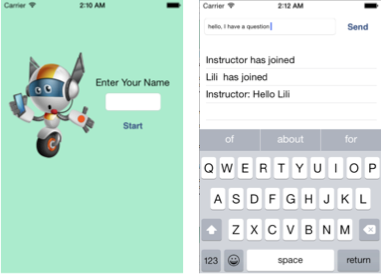
\includegraphics[height=2.0in, width=2.7in]{fig1}
\caption{An example of chat function in the application}
\end{figure}

\begin{figure}
\centering
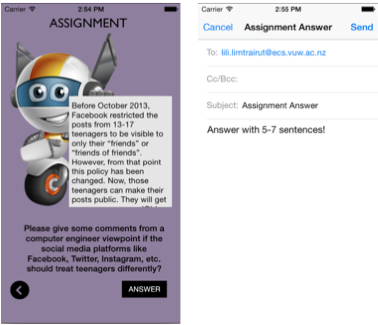
\includegraphics[height=2.0in, width=2.7in]{fig2}
\caption{An example of assignment given in the application}
\end{figure}

\begin{enumerate}
\item{\textbf{Chat}: An available communication channel for learners to contact their instructors. It supports both synchronous and asynchronous as well as a public mode (i.e., many learners and an instructor are in the same chat room) and a private mode (i.e., one-on-one communication between a learner and an instructor) communications. Figure 1 shows an example of asynchronous, public mode chat room design}
\item{\textbf{Media}: There are text, recorded audio, and video presentations available in the application, which are used to deliver learning contents
\item{\textbf{Game-based Learning}: An opportunity for learners to practice what they have learnt}
\item{\textbf{Assignment}: In order to improve learners' cognitive skills, we provided a short case study for them to read (Figure 2). It is compulsory that they answer (i.e., a short answer) the given question, send the answer to an instructor' email and they will receive feedback from the instructor}
}
\end{enumerate}



%%%%%%%%%%%%%%%%%%%%%%%%%%%%%%%%%%%%%%%%%%%%%%%%%%%%%%%%%%%%%%%%%%%
 
\section{RESEARCH METHODOLOGY}

\noindent We recruited first year computer engineering, and computer science students from School of Engineering and Computer Science, Victoria University of Wellington, New Zealand to participate in our online-based, anonymous questionnaire by sending a classless email. From an approximately 150 students, 30 of them completed the survey. 

Our participants were students who enrolled either in Engineering Modelling and Design or Introduction to Data Structures and Algorithm courses. We conducted the study on October, 2015 during second trimester. Our participants have passed at less one basic computer course, hence they had experience in learning in university. 

In order to create a persona, we adopted \citet{cooper2007face}, and \citet{mulder2006user}'s suggestions. \citet{cooper2007face} suggested seven principle steps (i.e., identify behavioral variables, map interview subjects to the variables, identify significant behavior patterns, synthesize characteristics and relevant goals, check for redundancy and completeness, expand description of attributes and behaviors, and designate persona types) while \citet{mulder2006user} suggested three types of research (i.e., Qualitative research, Qualitative research with quantitative validation, Quantitative research) that helped developers to create personas. 

There are two behavioral variables (i.e., experience, and attitude) that we observed. We adopted quantitative research to observe learners' experience in using mobile phones for both general and educational purposes, and learners' attitude towards m-learning, the given media and the given functions. Likert scale was used to rank the experience and measure the attitude. This could help us to predict if the given media and functions (e.g., video, recorded audio, chat) are practically possible to facilitate learning. 

We adopted qualitative research to observe what activities other than calling and texting learners performed using their mobile phones, how they used their mobile phones to support learning, and their goal of learning on mobile phones. Text box fields were used to collect free-form, text-based responses. 

In order to identify significant behavior patterns, we plotted the quantitative results into graphs and seek for learners' archetype. In the next section, we will present our persona, the process we used to find learners' behaviour patterns, and general findings from the survey. 

%%%%%%%%%%%%%%%%%%%%%%%%%%%%%%%%%%%%%%%%%%%%%%%%%%%%%%%%%%%%%
\section{RESULTS AND ANALYSIS} 

\noindent From a total of 30 participants, 26 are male students, and four are female students. The average age of participants is 22 year old. 

\subsection{Persona of M-Learning Learners}

\noindent We gathered all the results, categorized them, found a behavioural pattern, and created a persona (Figure 3). This persona will be used to represent our target learners by all people involved in this m-learning application development process. 
\begin{figure}
\centering
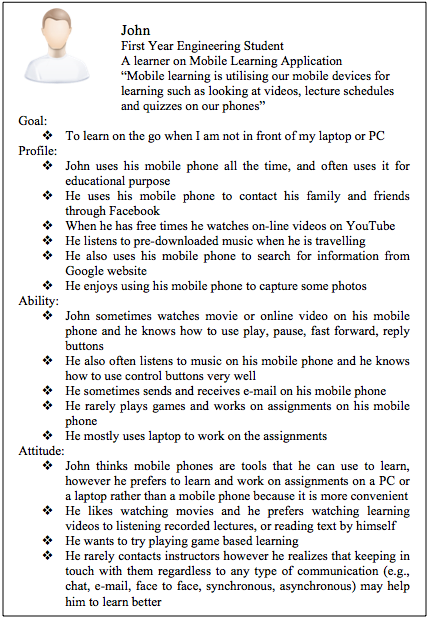
\includegraphics[height=3.8in, width=3in]{fig3}
\caption{Persona represents learners of m-learning application on mobile phones}
\end{figure}


\begin{figure}
\centering
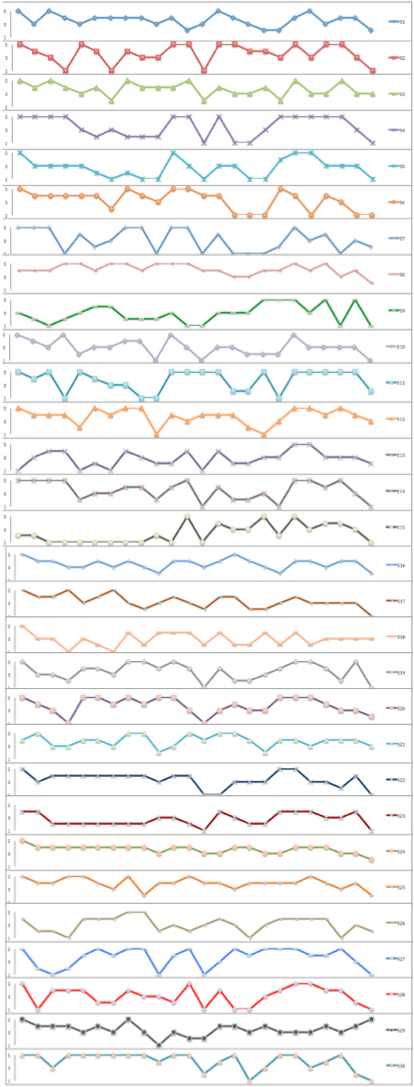
\includegraphics[height=7.6in, width=3in]{fig4}
\caption{The graph of 30 participants' responses to 24 quantitative questions plotted alongside each other. The x-axis presents the 24 qualitative questions, while the y-axis presents the level of learners' experience and attitude toward m-learning, the provided media and functions in the range one to five. We plotted this graph to see each individual's responses and the trend in graphs. However, it could not help us to find learners' behaviour pattern}
\end{figure}

This persona was created based on the results of participants' responses to 24 quantitative questions. In an attempt to find a behaviour pattern from these responses, we plotted them alongside each other (Figure 4). This graph helped us to see each individual trend clearly; however, it could not help us to find learners' behaviour pattern. 

\begin{figure}
\centering
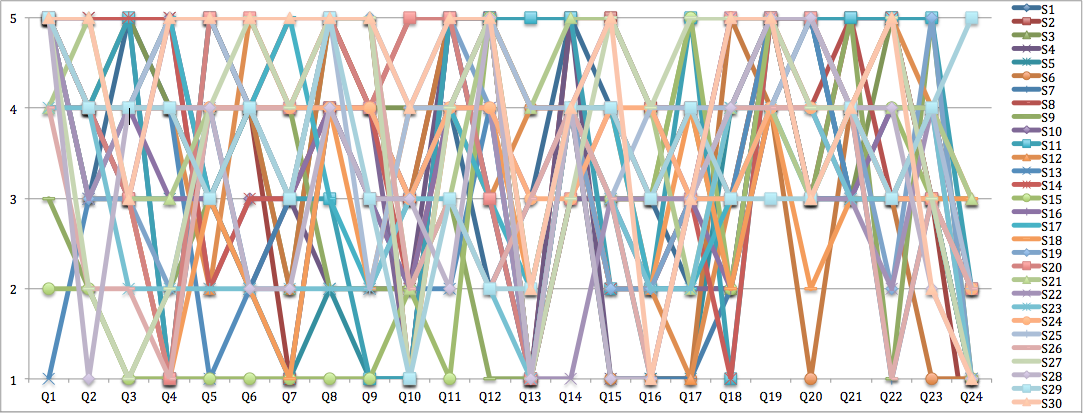
\includegraphics[height=1.7in, width=3in]{fig5}
\caption{This graph is the compressed 30 participants' responses (from Figure 4) in a single scale. The x-axis presents 24 quantitative questions, while the y-axis presents the responses in the range one to five}
\end{figure}

Next, we plotted them on the same graph (Figure 5). we found that the resulting graph was overly distributed and was not effective for determining learners' behaviour pattern, therefore we performed three rounds of clustering. 

\begin{figure}
\centering
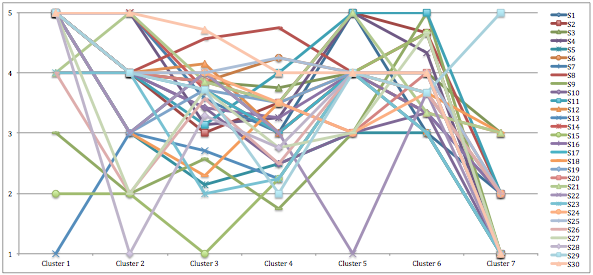
\includegraphics[height=1.7in, width=3in]{fig6}
\caption{The graph after first round attribute clustering. The x-axis presents seven clusters, while the y-axis presents the responses in the range one to five}
\end{figure}

\begin{figure}
\centering
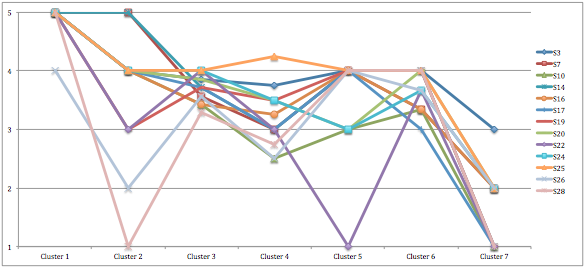
\includegraphics[height=1.7in, width=3in]{fig7}
\caption{The graph after second round interval cutting-off}
\end{figure}

\begin{figure}
\centering
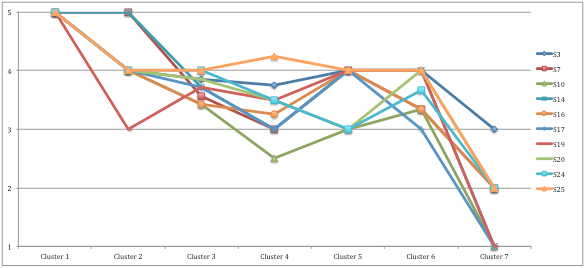
\includegraphics[height=1.7in, width=3in]{fig8}
\caption{The graph after third round the extreme value cutting-off}
\end{figure}

\begin{itemize} 
\item \textbf{First round attribute clustering}: The questions were divided into seven clusters (i.e., experience in using a mobile phone in daily life, experience in using a mobile phone for educational purpose, experience in using the provided media, experience in using the provided functions, attitude towards m-learning, attitude towards provided functions, and learning preference). For the clusters that consisted of more than one question, we plotted the graph based on their average values (Figure 6).


\item \textbf{Second round cutting off}: Based on the average values, we set an allowed interval for each cluster.  If a participant provided two or more responses outside the allowed interval, we cut through the participant off the considered group. There were 17 participants who were cut off in this round (Figure 7). 

\item \textbf{Third round cutting off due to the extreme value}: There were three participants who were qualified from the second round cutting off, but were excluded in this round, as their responses to one question varied greatly from other participants in the same cluster.

\end{itemize}

The final ten participants showed a similar trend. They were the archetype and we created a persona based on them. We assigned a pseudonym which was ``John'' to represent the persona. According to the participants' responses in Figure 8: 
\begin{itemize}
\item{\textbf{Cluster 1}: John ``all of the time'' uses his mobile phone for things other than calling and texting. We used a qualitative question to specify the activities and we found that John watched Videos on YouTube\footnote{https://www.youtube.com}, listened to pre-downloaded musics, went to Google\footnote{https://www.google.co.nz} website to search for some information, and used his mobile phone's camera to capture photoes. He also used his mobile phone to communicate with his friends and family.}
\item{\textbf{Cluster 2}: John ``often'' uses his mobile phone for educational purposes.  We also used a qualitative question to specify the educational activities. The answers were varied (e.g., he used his mobile phone's camera to capture lecture notes' photos, he went to school's website and viewed online learning contents on his mobile phone)}
\item{\textbf{Cluster 3}: John ``sometimes'' uses the media (i.e., video, recorded audio, and text) that we provided in the application (i.e., he sometimes watches videos, listenes to pre-downloaded musics, and read online articles)}
\item{\textbf{Cluster 4}: The responses in this cluster were varied between two (rarely performed the given tasks) to four (often performed the given tasks), therefore we could not form a behavior pattern based on the whole cluster. However, when we looked into each question (i.e., each given task) within this cluster, we found patterns (i.e., John ``sometimes'' uses his mobile phone to send/receive emails, he ``rarely'' plays games or works on an assignment on his mobile phone)}
\item{\textbf{Cluster 5}: John agreed that mobile phones have helped him in his learning}
\item{\textbf{Cluster 6}: John has positive attitude towards provided functions (e.g., he realizes that contacting instructors either face to face or via email have helped him to engage with learning)}
\item{\textbf{Cluster 7}: John prefers to learn on a laptop or PC rather than a mobile phone. Therefore, more encouragement and promotions may be required in order to increase the application's usage and recognition}
\end{itemize}

%%%%%%%%%%%%%%%%%%%%%%%%%%%%%%%%%%%%%%%%%%%%%%%%%%%%%%%%%%%%%%%%%%%
\subsection{General Findings}
\subsubsection{Learners' Experience in Using Mobile Phones for General and Educational Purposes}
\noindent We adopted Likert scale to measure how often (i.e., 1= never, 2 = rarely, 3 = sometimes, 4 = often, and 5 = all of the time) learners used their mobile phones in daily life, and whether they used it for educational purpose. Our findings (Table 1) shows that learners used their mobile phone ``all the time''. We also asked them to list the activities that they performed on their mobile phones other than calling and texting. The following list shows the usage categories. 
\begin{itemize}
\item{Communication purpose: They used their mobile phones to access social media websites (e.g., Facebook\footnote{https://www.facebook.com}, Reddit\footnote{https://www.reddit.com}, and sending and receiving e-mails}
\item{Entertainment purpose: They used their mobile phones to watch video online from video-sharing websites (e.g., YouTube), listen to music, and play games}
\item{Researching purpose: Participants mentioned that they accessed Google whenever they wanted to find any information. They also read news, and participated in online-forums on their mobile phones}
\item{Personal Management purpose: They used many basic functions available on their mobile phones to manage their daily life. For example, they used note function to list activities to be completed, used calendar to receive notifications regarding when these tasks should be completed, used alarm clock to wake them up in the morning and they managed their bank account online}
\item{Other purpose: They mentioned many others basic functions of mobile phones (e.g., flash light, map, camera) which they used regularly}
\end{itemize}
%%%%%%%%%%%%%%%%%%%%%%% TABLE 1%%%%%%%%%%%%%%%%%%%%%%%%%%%%%%%%%%%%%
\begin{table}
\centering
\caption{Learners' experience in using a mobile phone for general and educational purpose in their daily life}\
\begin{tabular}[BP]{ | p{3.5cm} | p{1.3cm} | p{1.3cm} |}
\hline Question & Mean & SD\\ 
\hline For things other than calls and texts & 4.53 & 0.97\\
\hline For educational purpose & 3.57 &1.04\\
\hline 
\end{tabular}
\end{table}

%%%%%%%%%%%%%%%%%%%%%%% TABLE 2 %%%%%%%%%%%%%%%%%%%%%%%%%%%%%%%%%%
\begin{table*}
\centering
\caption{Learners' experience in using a mobile phone to perform the given tasks}\
\begin{tabular}[BP]{ | p{11.0cm} | p{1.2cm} | p{1.2cm} |}
\hline Task & Mean & SD\\ 
\hline Reading long text such as an on-line article from the screen of mobile phone & 3.50 & 1.20\\
\hline Using a scroll-up and scroll-down bar to go through text & 3.17 & 1.53 \\
\hline Using zoom-in and zoom-out to read text & 3.43 &1.17\\
\hline Playing video on mobile phone & 3.50 & 1.11\\
\hline Using play, pause, rewind, fast forward, or repeat functions of video player & 3.03 &1.19\\
\hline Listening to recorded audio or music on mobile phone &4.00 &1.17\\
\hline Using play, pause, rewind, fast forward, or repeat functions of music player &3.37 &1.33\\
\hline Playing game on mobile phone &2.57 & 1.22\\
\hline Sending/Receiving e-mail on mobile phone & 3.97 &1.07\\
\hline Text chatting on mobile phone & 3.93 &1.23\\
\hline Doing homework/assignment on mobile phone&2.07&1.28\\
\hline
\end{tabular}
\end{table*}
%%%%%%%%%%%%%%%%%%%%%%%%%%%%%%%%%%%%%%%%%%%%%%%%%%%%%%%%%%%%%%%%%%%%%%%%%%%%%
When we specified the usage of mobile phones to \textbf{educational purposes}, the usage level was slightly decreased to ``often''. We also asked them to explain how they used their mobile phones to support their learning. The results show the same usage categories (listed previously) being applied by students in the educational context. The interesting findings are: 
\begin{itemize}
\item{They used their mobile phones to access to social media websites to contact their classmates and discuss their lessons and assignments}
\item{They also downloaded lecture notes, slides, and videos and used these downloaded materials from their mobile phones when they were outside university}
\item{For research purpose, they read articles on their mobile phones and used online search engines (i.e., Google) when they had questions and wanted to find more information}
\item{They visited the school's website to keep themselves updated, and accessed learning resources via University's Blackboard system}
\item{They used mobile phones' basic functions such as clock, calendar, and note to help them to manage their learning schedule, and they also used their camera to capture their lecture notes}
\end{itemize} 

Based on these findings, mobile phones are confirmed to be powerful tools for supporting ubiquitous learning. The use of mobile phones as an educational tool is now very much an established part of our target learners' daily learning environment. 

%%%%%%%%%%%%%%%%%%%%%%%%%%%%%%%%%%%%%%%%%%%%%%%%%%%%%%%%%%%%%%%%%%%%%%

\subsubsection{Learners' Goals toward M-Learning}
\noindent We asked learners to explain the term ``mobile learning''. Most of them showed that they understand the term. For example a student answered that 
\newline 
\newline 
\textit{``Mobile learning to me is being able to gain and apply knowledge anywhere at anytime including when an internet connection is unavailable''}
\newline 
\newline 
\indent The results showed that learners could differentiate m-learning from other types of learning. They mentioned learning on the go, learning anywhere, and convenient when they were not stationary. 

We asked learners to identify their goals of learning on mobile phone.  It appeared that they did not have a clear goal for m-learning. Most of them considered mobile phones as tools to help them to learn outside of their classrooms when they were not in front of their laptop and PC. Examples of the answers are: 
\newline 
\newline 
\textit{``I do not consider myself a person who learns from a mobile phone, only one who uses it for time management and organising my learning, which comes from other sources unless it is an extreme scenario (i.e. there are absolutely no computers available to me)''}
\newline
\newline 
\textit{``I just want to be able to find out what I need to know very quickly. I can do this already!''}
\newline 
\newline 
\indent These results pointed out that our target learners did not take m-learning as a primary source of learning and they did not set up a learning goal even though they adopted the phones for many learning activities. It raised awareness about learners' m-learning acceptance and that encouragement and promotions (e.g., use rewarding technique) may be required. 


%%%%%%%%%%%%%%%%%%%%%%%%%%%%TABLE3%%%%%%%%%%%%%%%%%%%%%%%%%%%%%%%%%%%%%%%%%%
\begin{table*}
\centering
\caption{Learners' attitude towards m-learning and the given functions}\
\begin{tabular}[BP]{ | p{12.0cm} | p{1cm} | p{1cm} |}
\hline Task & Mean & SD\\ 
\hline Mobile phone has helped me in my learning process & 3.87 & 0.82\\
\hline I prefer learning by watching a video on a mobile phone rather than reading text on a mobile phone& 3.10 & 1.27 \\
\hline I prefer learning by listening to a recorded audio on a mobile phone rather than reading text on a mobile phone & 2.43 &1.07\\
\hline I like game based learning activities & 3.30 & 1.22\\
\hline I feel frustrated typing on small key board of a mobile phone & 3.37 &1.27\\
\hline Assignments help me to improve my learning & 4.60 & 0.56 \\
\hline I prefer doing an assignment on a computer rather than writing on actual paper & 3.83 & 1.09\\
\hline Keeping in touch with my instructor can encourage me to learn & 3.83 & 0.70\\
\hline I prefer sending an e-mail or a message to my instructor rather than having a face-to-face conversation&3.43 &1.25\\
\hline I prefer having synchronous rather than asynchronous communication with instructor & 3.37 & 0.89\\
\hline I prefer learning on a mobile phone rather than learning on a laptop or a desktop computer & 1.17 &0.92\\
\hline
\end{tabular}
\end{table*}
%%%%%%%%%%%%%%%%%%%%%%%%%%%%%%%%%%%%%%%%%%%%%%%%%%%%%%%%%%%%%%%%%%%%%%%
\subsubsection{Learners' Experience in Using Provided Functions}
In this section, we observed if learners had experience in using the functions that we planed to provide in our application. We adopted Likert scale (i.e., 1= never, 2 = rarely, 3 = sometimes, 4 = often, and 5 = all of the time) to indicate how often they had performed the tasks. 

As outlined in our results collated in Table 2, learners pointed out that they ``sometimes'' to ``often'' perform the given tasks. Base on these results, learners should be able to learn by reading text, watching video presentation, and listening to recorded audio. If they have questions, want to share their ideas, or discuss their ideas with instructor they should be able to use the provided communication channels (e.g., sending an e-mail to instructor, entering chat room).

On the other hand, they expressed that they ``rarely'' played games and worked on assignments on their mobile phones. These findings raised some concerns that they might not play the provided game-based learning and submit the given assignment. We may need to find strategies to promote our game-based learning (e.g., arrange competitions in which highest score winners receive rewards). For the assignment, we may need to arrange a submission deadline or use rewarding technique to encourage their participations. 

%%%%%%%%%%%%%%%%%%%%%%%%%%%%%%%%%%%%%%%%%%%%%%%%%%%%%%%%%%%%%%%%%%%%%%%%%%%%%%%%%%%%%%%%%%%%%%%%%%%%%%%%%%%%%%%%%%%%%%%%%%%%%%%%%%%%%%%%%%%%%%%%
\subsubsection{Learners' Attitude toward M-Learning}
We observed learners' attitude toward m-learning and the functions that we planed to develop in the application. We adopted Likert scale (i.e., 1= strongly disagree, 2 = disagree, 3 = neutral, 4 = agree, and 5 = strongly agree) to indicate how much they agreed with the given statement. Table 3 presents the results. 

Based on the results in Table 3, learners showed that they had positive attitudes toward using mobile phones to support their learning process. They further indicated that learning through video presentation was the most popular learning style, followed by learning by reading text. Even though they expressed that they had the most experience listening to recorded audio or music, they preferred it the least. 

For game based learning, they expressed that they did not have negative nor positive attitudes toward them even though they rarely played games on mobile phones. 

Learners ``strongly agree'' that assignments had helped them to improve their learning and they preferred performing them on a computer rather than on actual paper, hence assignments showed high potential for improving learning quality and should be added into m-learning application. However, students expressed that they felt frustrated typing using small mobile phone keyboards, therefore the given assignment in the application should be short answers, or multiple choices types of questions. 

For communication, learners agreed that keeping in touch with instructors could encourage them to learn and they slightly preferred sending e-mail or message to instructor rather than having a face-to-face conversation. Similarly, they slightly preferred synchronous to asynchronous communication. 

Lastly, even though learners had positive attitude towards using mobile phones to support their learning, they still preferred to learn on a laptop or a desktop computer rather than on a mobile phone. This could be an effect of hardware limitations (e.g., small size keyboard, screen, low solution). 


%%%%%%%%%%%%%%%%%%%%%%%%%%%%%%%%%%%%%%%%%%%%%%%%%%%%%%%%%%%%%%%%%%%%%%%
\section{CONCLUSIONS} 
\noindent Distance learning may trigger feelings of isolation or perceived emptiness in learners as they have to exercise more self-discipline and control over their one learning. Transaction Distance Theory suggested how distance education should be constructed. Grounded on this theory, we designed an m-learning application. We observed whether this theoretical-based design is practically possible for our target learners. 

A total of 30 participants, 26 male and four female, who are first year computer engineering and computer science students at Victoria University of Wellington, New Zealand answered an online-based questionnaire. The significant findings are: 
\begin{itemize} 
\item{Our target learners had a lot of experience in using mobile phones. They used them as communication tools (e.g., access to social media, chatting), entertainment tools (e.g., watch video, listen to music), researching tools (e.g., access to Google), and management tools (e.g., set up notification, alarm clock)} 
\item {Our target learners often used their mobile phone for educational purposes}
\item {Our target learners knew what m-learning was, but they did not have a cleared goal towards m-learning} 
\item {Our target learners had experience in using the provided media (i.e., text, video, recorded audio) and they preferred to learn from video presentation rather than reading text, and listening the recorded audio} 
\item{Our target learners had a lot of experience in using the chat function but they had less experience playing game, and working on their assignments on mobile phones} 
\item {Our target learners had positive attitudes towards m-learning, however they preferred learning on a laptop or a desktop computer rather than learning on a mobile phone}
\end{itemize} 

Based on these findings, our Transactional Distance Theory-based design was practically appropriate for our learners. They should be able to learn from provided media, and be able to use the provided chat function to communication with instructors. However, we need to find strategies to encourage learners to participate in the game-based learning, and complete the given assignment. We can use rewarding techniques and send assignments notifications to them. 

Our survey results also indicated that our learners did not consider m-learning on mobile phones as their major learning source. In order to increase application usage, m-learning needs more promotions and encouragement. 

Finally, we created a persona based upon learners' archetype, which will be shared among the people involved in this application development process. 

%%%%%%%%%%%%%%%%%%%%%%%%%%%%%%%%%%%%%%%%%%%%%%%%%%%%%%%%%%%%%%%%%%%%%%

\vfill
\bibliographystyle{apalike}
{\small
\bibliography{example}}

\vfill
\end{document}

